\documentclass[12pt]{jhwhw}
\author{Ian Malerich}
\title{Math 424 - Lab 14}
\usepackage{amssymb, amsfonts, mathtools, graphicx, breqn, subfig}
\usepackage{minted, subfig, float, scrextend, setspace}
\usemintedstyle{friendly}

\DeclarePairedDelimiter\ceil{\lceil}{\rceil}

\onehalfspacing
\begin{document}
\raggedright

%% Chapter 3 starts on page 104
%% Exercises start on page 161

\textbf{3.6}
	Suppose \textit{comm\_sz=4} and suppose that $x$ is a vector with $n=14$ 
	components.
	\begin{enumerate}
		\item How would the components of $x$ be distributed among the processes in 
			a program that used a block distribution.
		\item How would the components of $x$ be distributed in a process that 
			used a cyclic distribution?
		\item How would the components of $x$ be distributed among the processes
			in a program that used a block-cyclic distribution with block size
			$b=2$.
	\end{enumerate}
\textcolor[RGB]{240,240,240}{\rule{\textwidth}{0.5pt}}\bigbreak
	
	\begin{centering}
	\begin{tabular}{|l|c|c|c|c|}
		\hline
		\multicolumn{5}{|l|}{(a) Block} \\ \hline
		$P_0$ & 0 & 1 & 2 & 3 \\ \hline
		$P_1$ & 4 & 5 & 6 & 7 \\ \hline
		$P_2$ & 8 & 9 & 10 & 11 \\ \hline
		$P_3$ & 12 & 13 & &  \\ \hline
	\end{tabular}

	\smallbreak
	\begin{tabular}{|l|c|c|c|c|}
		\hline
		\multicolumn{5}{|l|}{(b) Cyclic} \\ \hline
		$P_0$ & 0 & 4 & 8 & 12 \\ \hline
		$P_1$ & 1 & 5 & 9 & 13 \\ \hline
		$P_2$ & 2 & 6 & 10 &  \\ \hline
		$P_3$ & 3 & 7 & 11 &  \\ \hline
	\end{tabular}

	\smallbreak
	\begin{tabular}{|l|c|c|c|c|}
		\hline
		\multicolumn{5}{|l|}{(c) Block Cyclic: b=2} \\ \hline
		$P_0$ & 0 & 1 & 8 & 9 \\ \hline
		$P_1$ & 2 & 3 & 10 & 11 \\ \hline
		$P_2$ & 4 & 5 & 12 & 13 \\ \hline
		$P_3$ & 6 & 7 & &  \\ \hline
	\end{tabular}

	\end{centering}

\clearpage
\textbf{3.8}
	Suppose \textit{comm\_sz=8} and $n=16$.
	\begin{enumerate}
		\item Draw a diagram that shows how MPI\_Scatter can be implemented using
			tree-structured communication on with comm\_sz processes when process 0
			needs to distribute an array containing $n$ elements.
		\item Draw a diagram that shows how MPI\_Gather can be implemented using 
			tree-structured communication when an n-element array that has been
			distributed among comm\_sz processes needs to be gathered into process 0.
	\end{enumerate}
\textcolor[RGB]{240,240,240}{\rule{\textwidth}{0.5pt}}\bigbreak

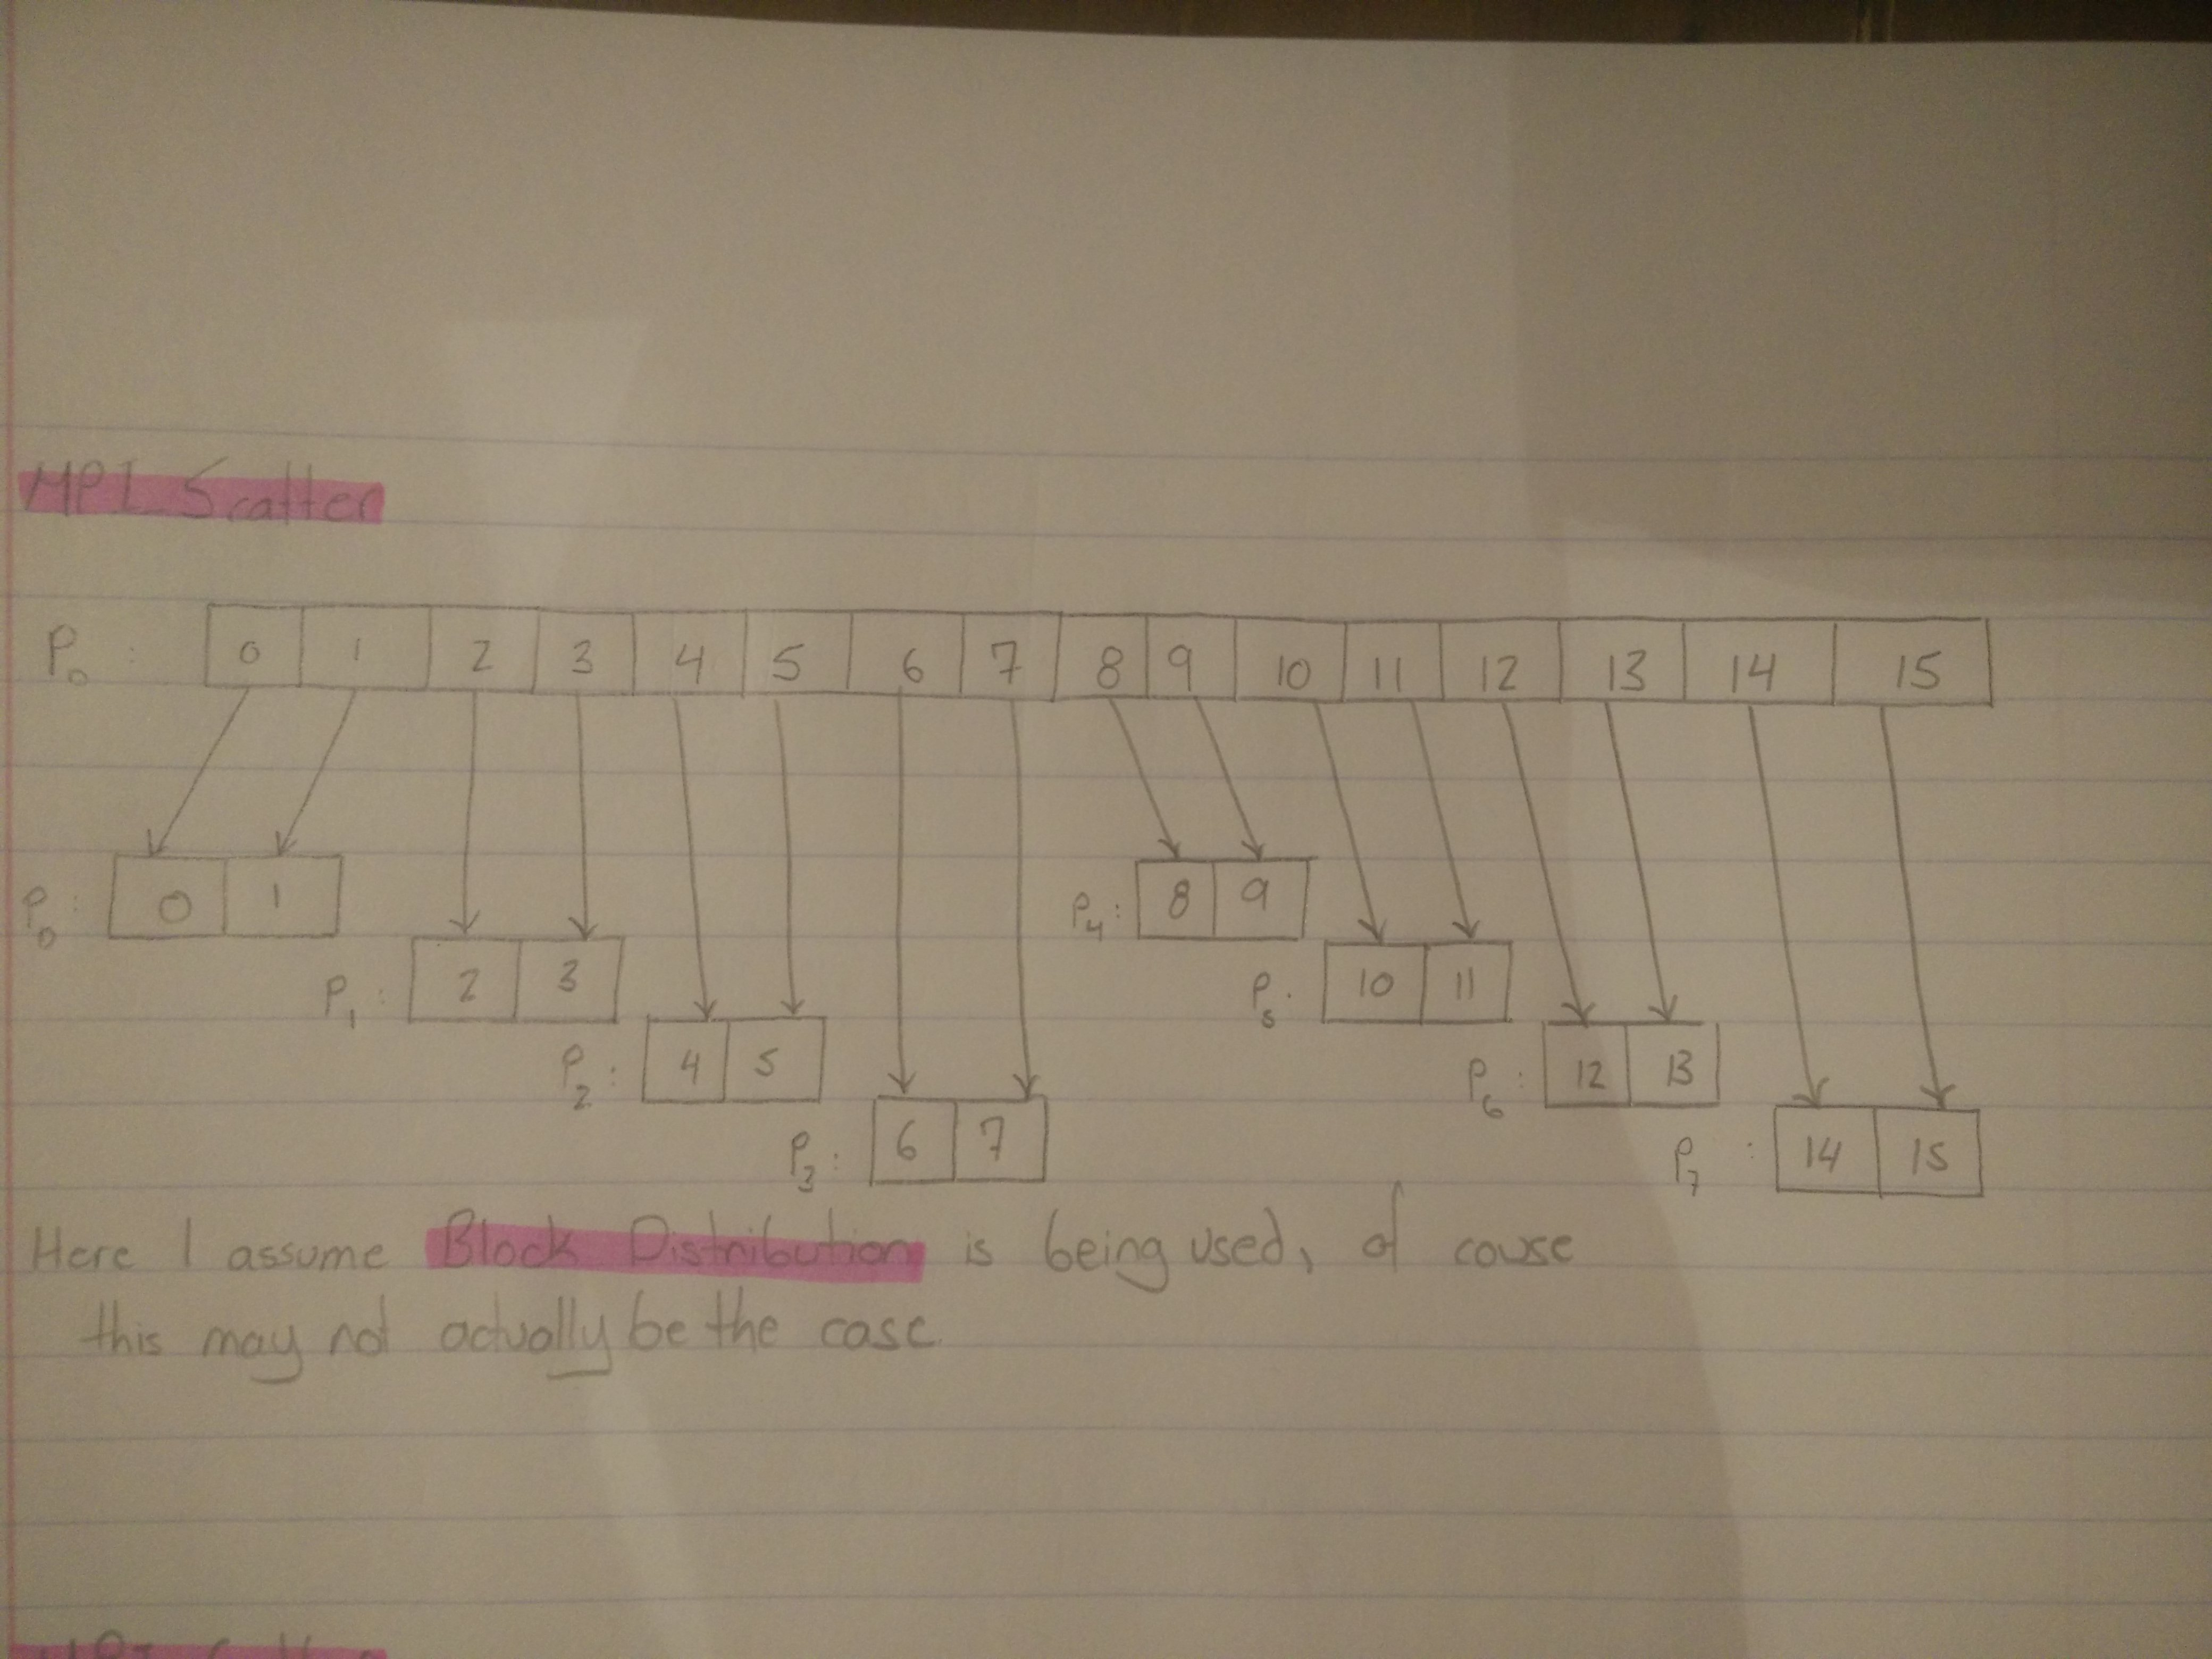
\includegraphics[scale=0.12]{MPI_Scatter.jpg}
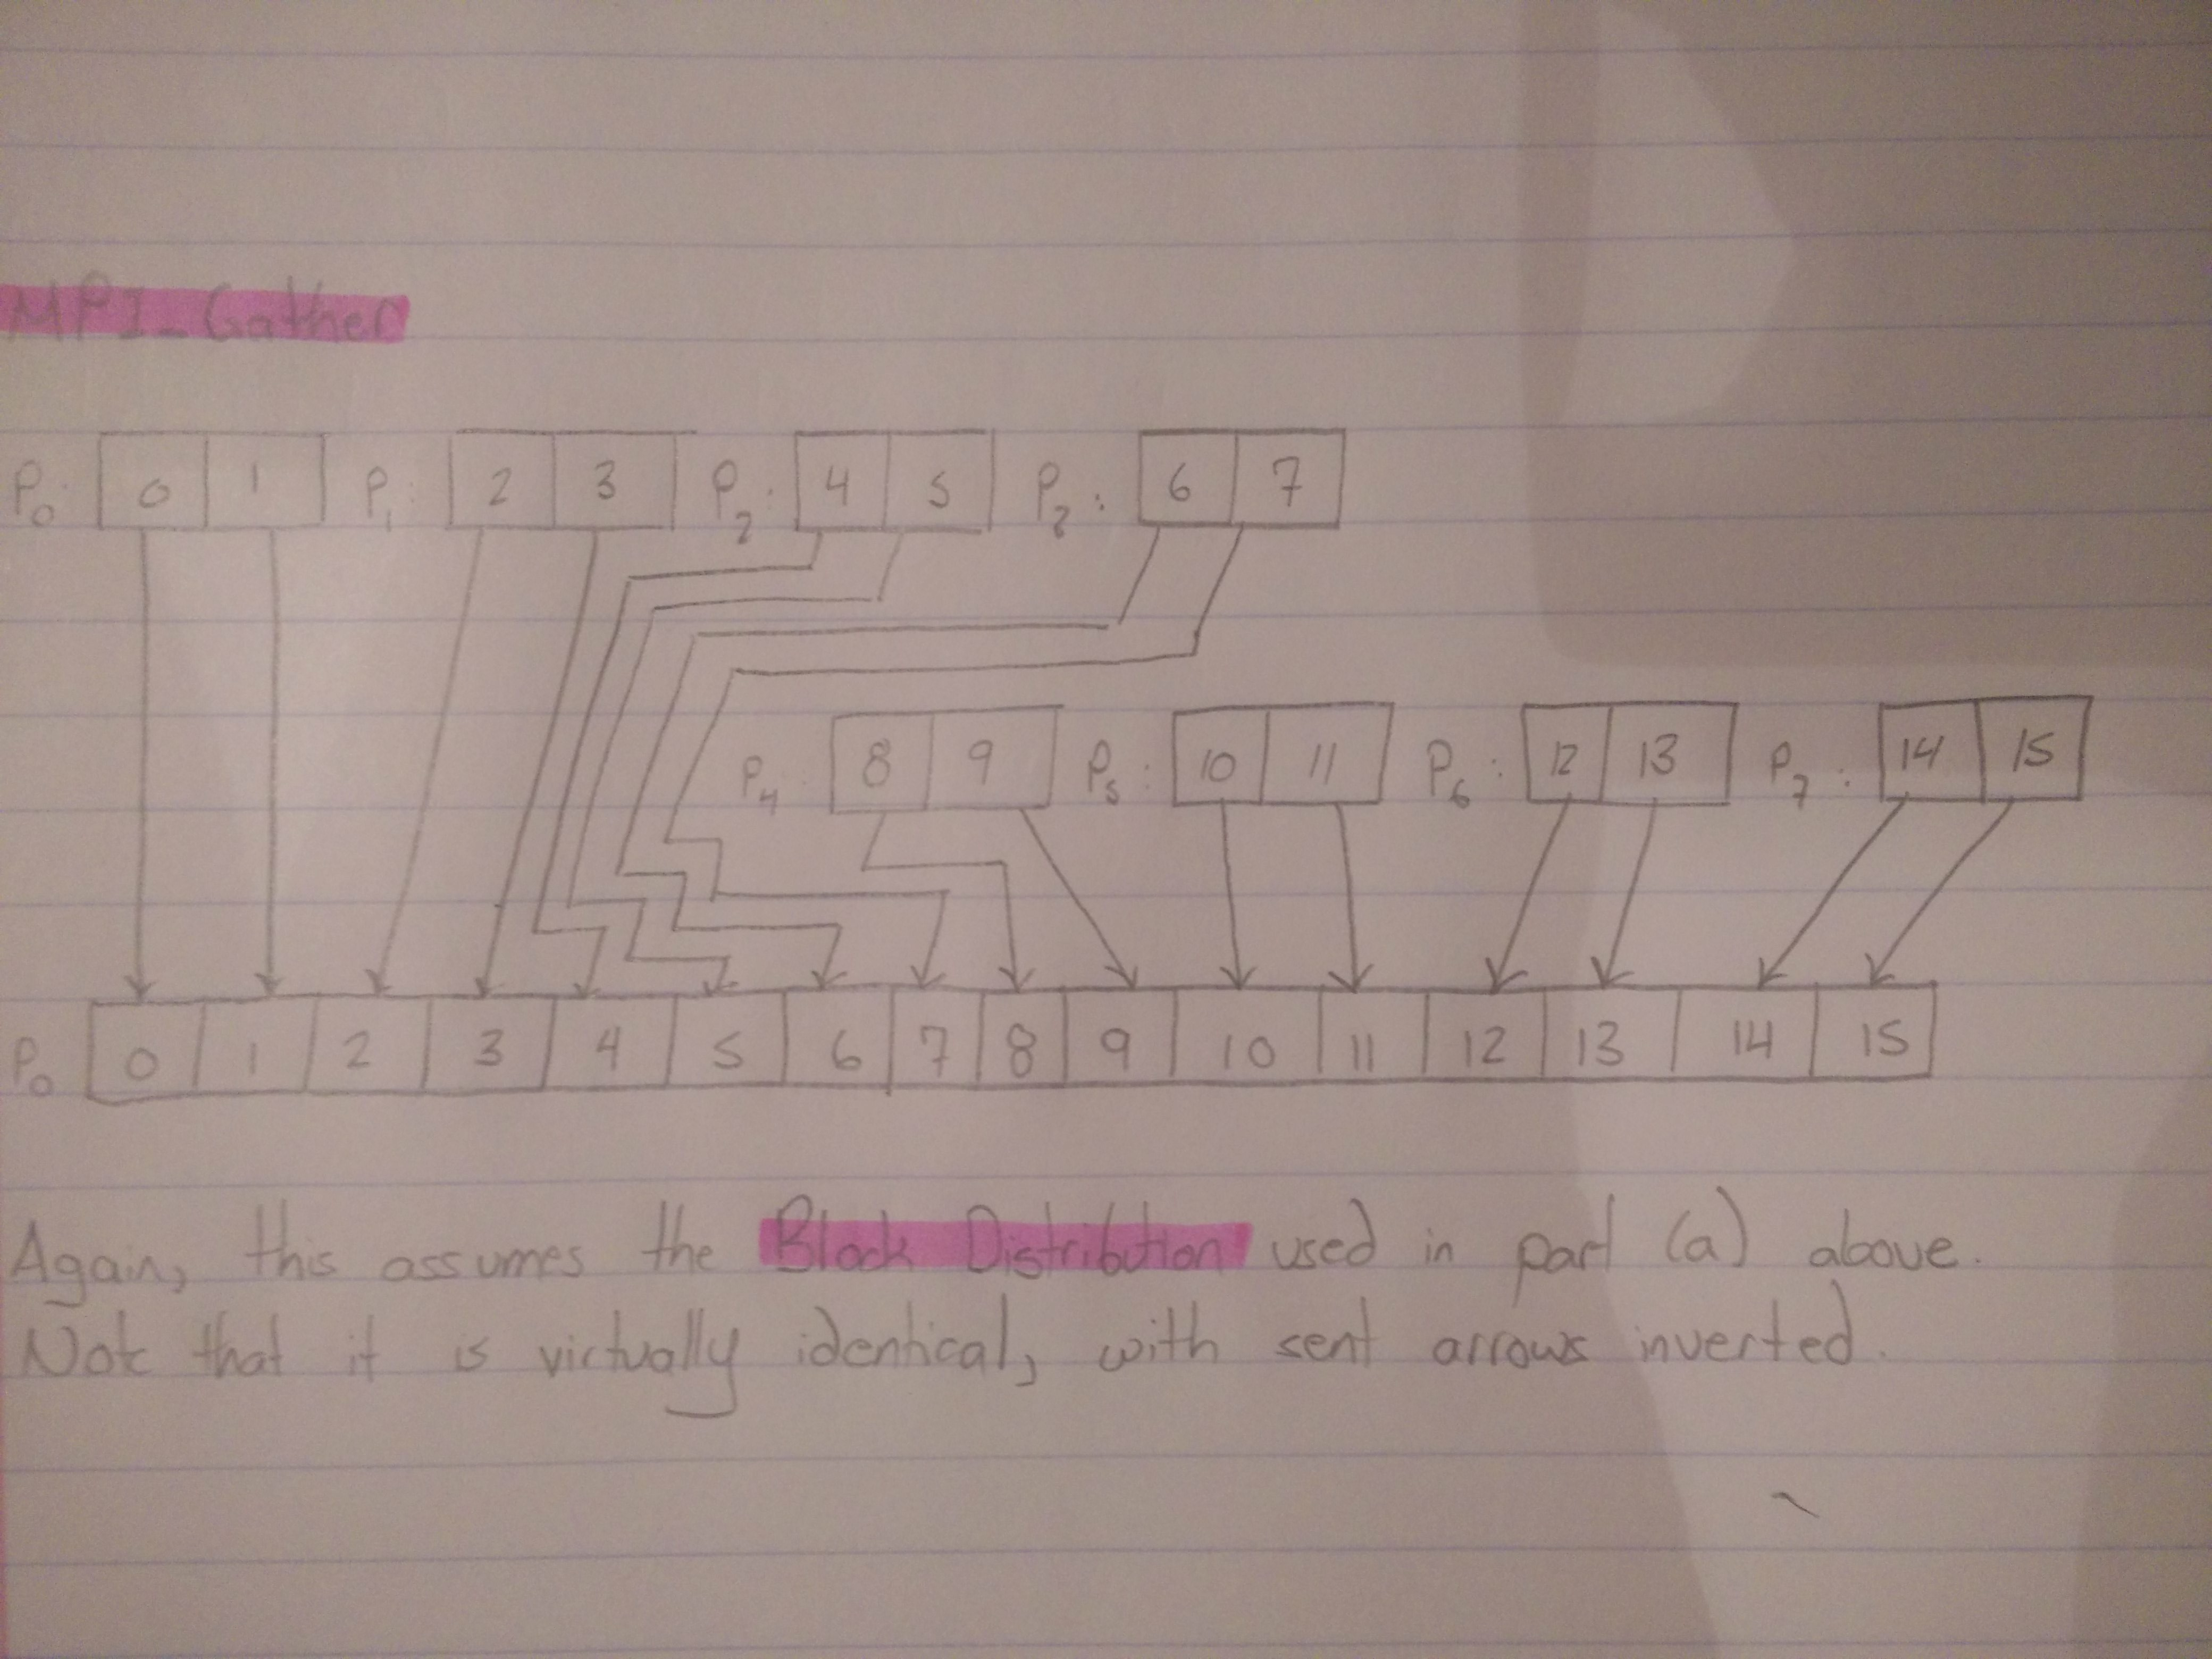
\includegraphics[scale=0.12]{MPI_Gather.jpg}

\clearpage
\textbf{3.9}
	Write an MPI program that implements multiplication of a vector by a scalar
	and dot product. The user should enter two vectors and a scalar, all of which
	are read in by process 0 and distributed among the processes. The results
	are calculated and collected onto process 0, which prints them.
	You can assume that n, the order of the vectors, is evenly divisible by 
	comm\_sz.
\textcolor[RGB]{240,240,240}{\rule{\textwidth}{0.5pt}}\bigbreak

\inputminted{c}{3.9.c}

\end{document}
